\documentclass[11pt,a4paper]{report}
\usepackage[textwidth=37em,vmargin=30mm]{geometry}
\usepackage{calc,xunicode,amsmath,amssymb,paralist,enumitem,tabu,booktabs,datetime2,xeCJK,xeCJKfntef,listings}
\usepackage{tocloft,fancyhdr,tcolorbox,xcolor,graphicx,eso-pic,xltxtra,xelatexemoji}

\newcommand{\envyear}[0]{2025}
\newcommand{\envdatestr}[0]{2025-08-29}
\newcommand{\envfinaldir}[0]{webdb/2025/20250829/final}

\usepackage[hidelinks]{hyperref}
\hypersetup{
    colorlinks=false,
    pdfpagemode=FullScreen,
    pdftitle={Web Digest - \envdatestr}
}

\setlength{\cftbeforechapskip}{10pt}
\renewcommand{\cftchapfont}{\rmfamily\bfseries\large\raggedright}
\setlength{\cftbeforesecskip}{2pt}
\renewcommand{\cftsecfont}{\sffamily\small\raggedright}

\setdefaultleftmargin{2em}{2em}{1em}{1em}{1em}{1em}

\usepackage{xeCJK,xeCJKfntef}
\xeCJKsetup{PunctStyle=plain,RubberPunctSkip=false,CJKglue=\strut\hskip 0pt plus 0.1em minus 0.05em,CJKecglue=\strut\hskip 0.22em plus 0.2em}
\XeTeXlinebreaklocale "zh"
\XeTeXlinebreakskip = 0pt


\setmainfont{Brygada 1918}
\setromanfont{Brygada 1918}
\setsansfont{IBM Plex Sans}
\setmonofont{JetBrains Mono NL}
\setCJKmainfont{Noto Serif CJK SC}
\setCJKromanfont{Noto Serif CJK SC}
\setCJKsansfont{Noto Sans CJK SC}
\setCJKmonofont{Noto Sans CJK SC}

\setlength{\parindent}{0pt}
\setlength{\parskip}{8pt}
\linespread{1.15}

\lstset{
	basicstyle=\ttfamily\footnotesize,
	numbersep=5pt,
	backgroundcolor=\color{black!5},
	showspaces=false,
	showstringspaces=false,
	showtabs=false,
	tabsize=2,
	captionpos=b,
	breaklines=true,
	breakatwhitespace=true,
	breakautoindent=true,
	linewidth=\textwidth
}






\newcommand{\coverpic}[2]{
    % argv: itemurl, authorname
    Cover photo by #2~~(\href{#1}{#1})
}
\newcommand{\makeheader}[0]{
    \begin{titlepage}
        % \newgeometry{hmargin=15mm,tmargin=21mm,bmargin=12mm}
        \begin{center}
            
            \rmfamily\scshape
            \fontspec{BaskervilleF}
            \fontspec{Old Standard}
            \fontsize{59pt}{70pt}\selectfont
            WEB\hfill DIGEST
            
            \vfill
            % \vskip 30pt
            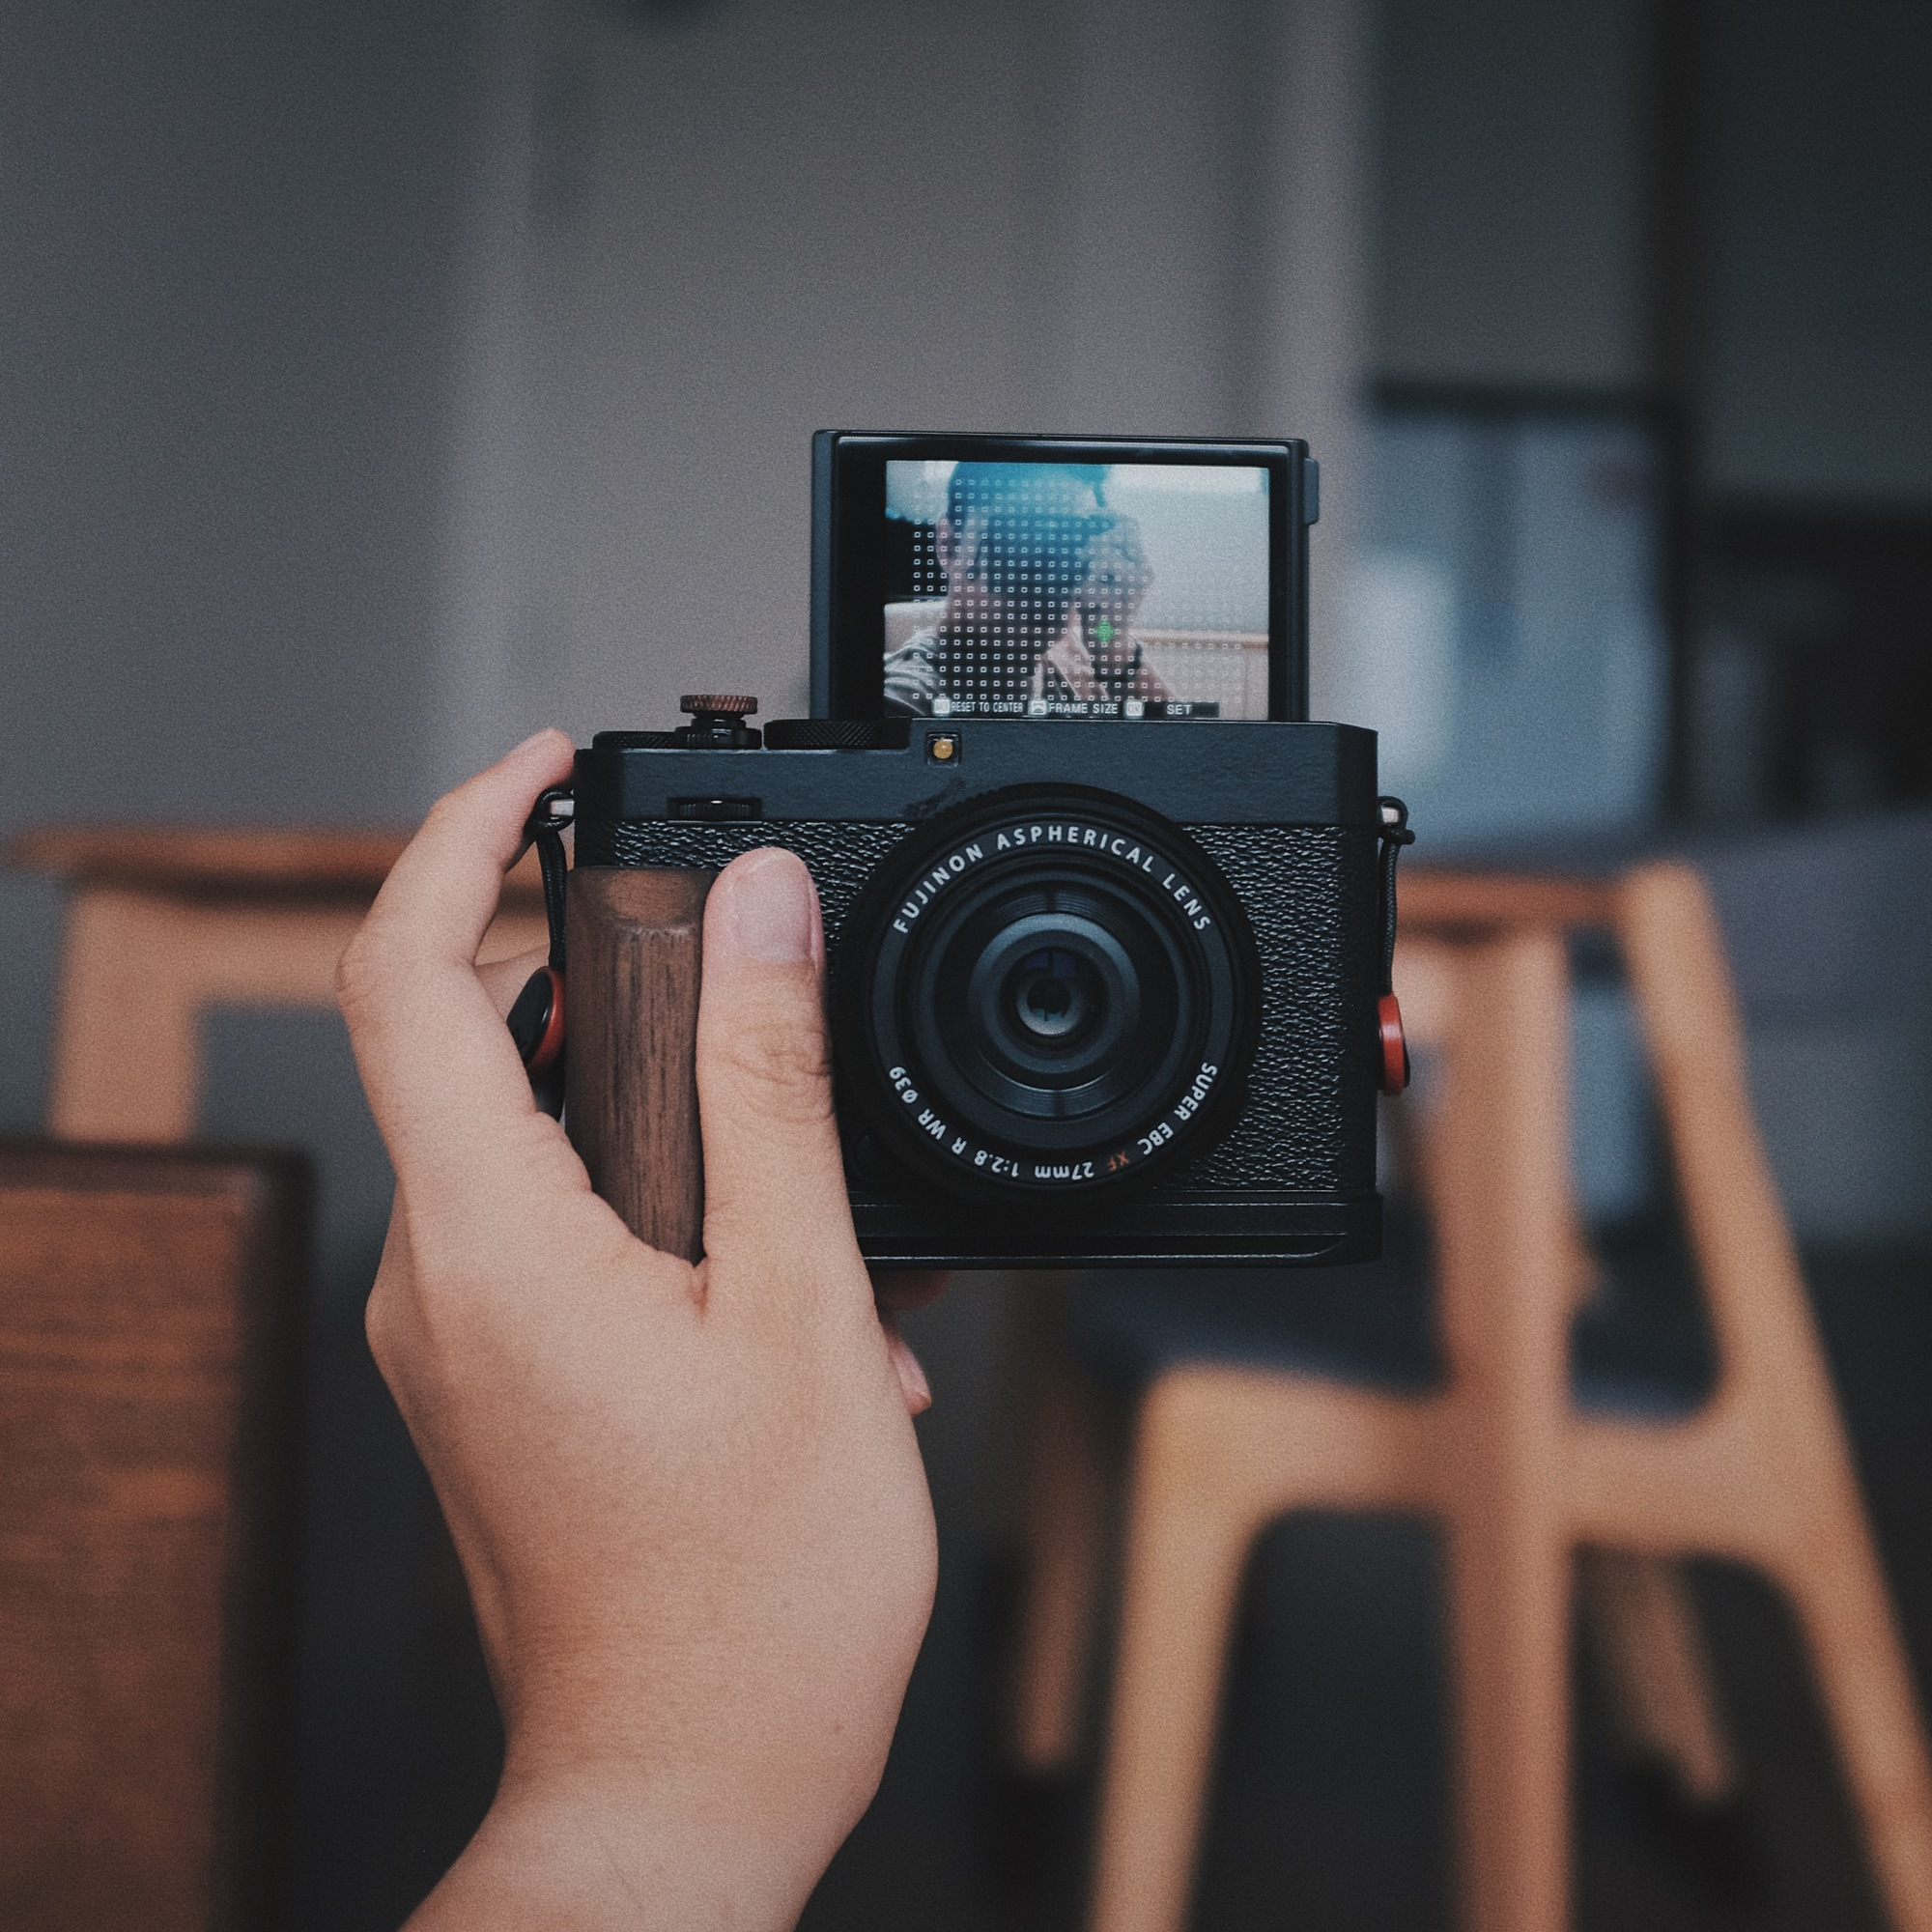
\includegraphics[width=\linewidth]{\envfinaldir/coverpic-prod.jpg}\par
            % \vskip 30pt
            \vfill

            \normalsize\rmfamily\scshape
            \copyright{} The Web Digest Project \hfill\large \envdatestr
        \end{center}
    \end{titlepage}
    % \restoregeometry
}
\newcommand{\simplehref}[1]{%
    \textcolor{blue!80!green}{\href{#1}{#1}}%
}
\renewcommand{\contentsname}{\center\Huge\sffamily\bfseries Contents\par\vskip 20pt}
\newcounter{ipartcounter}
\setcounter{ipartcounter}{0}
\newcommand{\ipart}[1]{
    % \vskip 20pt
    \clearpage
    \stepcounter{ipartcounter}
    \phantomsection
    \addcontentsline{toc}{chapter}{#1}
    % \begin{center}
    %     \Huge
    %     \sffamily\bfseries
    %     #1
    % \end{center}
    % \vskip 20pt plus 7pt
}
\newcounter{ichaptercounter}
\setcounter{ichaptercounter}{0}
\newcommand{\ichapter}[1]{
    % \vskip 20pt
    \clearpage
    \stepcounter{ichaptercounter}
    \phantomsection
    \addcontentsline{toc}{section}{\numberline{\arabic{ichaptercounter}}#1}
    \begin{center}
        \Huge
        \sffamily\bfseries
        #1
    \end{center}
    \vskip 20pt plus 7pt
}
\newcommand{\entrytitlefont}[1]{\subsection*{\raggedright\Large\sffamily\bfseries#1}}
\newcommand{\entryitemGeneric}[2]{
    % argv: title, url
    \parbox{\linewidth}{
        \entrytitlefont{#1}\par\vskip 5pt
        \footnotesize\ttfamily\mdseries
        \simplehref{#2}
    }\vskip 11pt plus 11pt minus 1pt
}
\newcommand{\entryitemGithub}[3]{
    % argv: title, url, desc
    \parbox{\linewidth}{
        \entrytitlefont{#1}\par\vskip 5pt
        \footnotesize\ttfamily\mdseries
        \simplehref{#2}\par\vskip 5pt
        \small\rmfamily\mdseries#3
    }\vskip 11pt plus 11pt minus 1pt
}
\newcommand{\entryitemAp}[3]{
    % argv: title, url, desc
    \parbox{\linewidth}{
        \entrytitlefont{#1}\par\vskip 5pt
        \footnotesize\ttfamily\mdseries
        \simplehref{#2}\par\vskip 5pt
        \small\rmfamily\mdseries#3
    }\vskip 11pt plus 11pt minus 1pt
}
\newcommand{\entryitemHackernews}[3]{
    % argv: title, hnurl, rawurl
    % \parbox{\linewidth}{
    %     \entrytitlefont{#1}\par\vskip 5pt
    %     \footnotesize\ttfamily\mdseries
    %     \simplehref{#3}\par
    %     \textcolor{black!50}{\href{#2}{#2}}
    % }\vskip 11pt plus 11pt minus 1pt
    \begin{minipage}{\linewidth}
            \entrytitlefont{#1}\par\vskip 5pt
            \footnotesize\ttfamily\mdseries
            \simplehref{#3}\par
            \textcolor{black!50}{\href{#2}{#2}}
    \end{minipage}\par\vskip 11pt plus 11pt minus 1pt
}







\begin{document}

\makeheader

\tableofcontents\clearpage




\ipart{Developers}
\ichapter{Hacker News}
\entryitemTwoLinks{My startup banking story (2023)}{https://news.ycombinator.com/item?id=45056177}{https://mitchellh.com/writing/my-startup-banking-story}

\entryitemTwoLinks{Some thoughts on LLMs and software development}{https://news.ycombinator.com/item?id=45055641}{https://martinfowler.com/articles/202508-ai-thoughts.html}

\entryitemTwoLinks{Uncertain<T>}{https://news.ycombinator.com/item?id=45054703}{https://nshipster.com/uncertainty/}

\entryitemTwoLinks{Ask HN: The government of my country blocked VPN access. What should I use?}{https://news.ycombinator.com/item?id=45054260}{https://news.ycombinator.com/item?id=45054260}

\entryitemTwoLinks{Service members deserve the right to repair}{https://news.ycombinator.com/item?id=45054037}{https://www.militarytimes.com/opinion/2025/07/11/why-service-members-deserve-the-right-to-repair/}

\entryitemTwoLinks{PinePhone Pro [GNU/Linux smartphone] has been discontinued}{https://news.ycombinator.com/item?id=45053872}{https://social.treehouse.systems/@pine64/115027515081143369}

\entryitemTwoLinks{China is eating the world}{https://news.ycombinator.com/item?id=45053771}{https://apropos.substack.com/p/china-is-eating-the-world}

\entryitemTwoLinks{Anything can be a message queue if you use it wrongly enough (2023)}{https://news.ycombinator.com/item?id=45053234}{https://xeiaso.net/blog/anything-message-queue}

\entryitemTwoLinks{Mosh Mobile Shell}{https://news.ycombinator.com/item?id=45053040}{https://mosh.org}

\entryitemTwoLinks{How to install TrueNAS on a Raspberry Pi}{https://news.ycombinator.com/item?id=45052429}{https://www.jeffgeerling.com/blog/2025/how-install-truenas-on-raspberry-pi}

\entryitemTwoLinks{AI adoption linked to 13\% decline in jobs for young U.S. workers: study}{https://news.ycombinator.com/item?id=45052423}{https://www.cnbc.com/2025/08/28/generative-ai-reshapes-us-job-market-stanford-study-shows-entry-level-young-workers.html}

\entryitemTwoLinks{Rendering a game in real time with AI}{https://news.ycombinator.com/item?id=45051188}{https://blog.jeffschomay.com/rendering-a-game-in-real-time-with-ai}

\entryitemTwoLinks{Charting Form Ds to roughly see the state of venture capital ``fund'' raising}{https://news.ycombinator.com/item?id=45051034}{https://tj401.com/blog/formd/index.html}

\entryitemTwoLinks{The Math Behind GANs (2020)}{https://news.ycombinator.com/item?id=45050958}{https://jaketae.github.io/study/gan-math/}

\entryitemTwoLinks{Important machine learning equations}{https://news.ycombinator.com/item?id=45050931}{https://chizkidd.github.io//2025/05/30/machine-learning-key-math-eqns/}

\entryitemTwoLinks{Microbial metabolite repairs liver injury by restoring hepatic lipid metabolism}{https://news.ycombinator.com/item?id=45050873}{https://journals.asm.org/doi/10.1128/mbio.01718-25}

\entryitemTwoLinks{Fossjobs: A job board for Free and Open Source jobs}{https://news.ycombinator.com/item?id=45050538}{https://www.fossjobs.net/}

\entryitemTwoLinks{Petition to stop Google from restricting sideloading and FOSS apps}{https://news.ycombinator.com/item?id=45050502}{https://news.ycombinator.com/item?id=45050502}

\entryitemTwoLinks{Are OpenAI and Anthropic losing money on inference?}{https://news.ycombinator.com/item?id=45050415}{https://martinalderson.com/posts/are-openai-and-anthropic-really-losing-money-on-inference/}

\entryitemTwoLinks{Windows 11 Update KB5063878 Causing SSD Failures}{https://news.ycombinator.com/item?id=45050192}{https://old.reddit.com/r/msp/comments/1n1sgxx/windows\_11\_update\_kb5063878\_causing\_ssd\_failures/}


\ipart{Developers~~~~(zh-Hans)}
\ichapter{Solidot}
\entryitemGeneric{\hskip 0pt{}用流行病学分析法国大革命}{https://www.solidot.org/story?sid=82168}

\entryitemGeneric{\hskip 0pt{}开源项目通常由一个人维护}{https://www.solidot.org/story?sid=82167}

\entryitemGeneric{\hskip 0pt{}Nothing 成为最新一家被发现用图库照片演示手机摄影能力的厂商}{https://www.solidot.org/story?sid=82166}

\entryitemGeneric{\hskip 0pt{}源自 ChatGPT 的常用词在人们的日常对话中也日益流行}{https://www.solidot.org/story?sid=82165}

\entryitemGeneric{\hskip 0pt{}三名台积电工程师因窃取 2 纳米工艺机密被起诉}{https://www.solidot.org/story?sid=82164}

\entryitemGeneric{\hskip 0pt{}印度屏蔽 Sci-Hub}{https://www.solidot.org/story?sid=82163}

\entryitemGeneric{\hskip 0pt{}《K-POP:猎魔女团》成为 Netflix 史上观看次数最多的电影}{https://www.solidot.org/story?sid=82162}

\entryitemGeneric{\hskip 0pt{}Windows 版本的 Word v2509 默认将文档保存到云端}{https://www.solidot.org/story?sid=82161}

\entryitemGeneric{\hskip 0pt{}GMP 项目报告 AMD CPU 烧毁事故}{https://www.solidot.org/story?sid=82160}

\entryitemGeneric{\hskip 0pt{} 开发者创新盛典 | NVIDIA 2025 Hackathon 年度总决赛报名即日启动!}{https://www.solidot.org/story?sid=82159}

\entryitemGeneric{\hskip 0pt{}韩国禁止中小学生课堂使用手机}{https://www.solidot.org/story?sid=82156}

\entryitemGeneric{\hskip 0pt{}Bluesky 成为科学社区的首选平台}{https://www.solidot.org/story?sid=82155}

\entryitemGeneric{\hskip 0pt{}AMD 称部分 X3D 烧毁是主板导致的}{https://www.solidot.org/story?sid=82153}

\entryitemGeneric{\hskip 0pt{}森林砍伐过去 20 年导致 50 万人死亡}{https://www.solidot.org/story?sid=82152}

\entryitemGeneric{\hskip 0pt{}Google 在翻译应用中加入 AI 驱动的语言学习功能}{https://www.solidot.org/story?sid=82151}

\entryitemGeneric{\hskip 0pt{}父母指控 OpenAI 的 ChatGPT 杀死了他们的孩子}{https://www.solidot.org/story?sid=82150}

\entryitemGeneric{\hskip 0pt{}苹果讨论过收购 Mistral AI 和 Perplexity}{https://www.solidot.org/story?sid=82149}

\entryitemGeneric{\hskip 0pt{}Anthropic 与图书作者就侵犯版权达成和解}{https://www.solidot.org/story?sid=82148}

\entryitemGeneric{\hskip 0pt{}无印良品在华商标诉讼败诉}{https://www.solidot.org/story?sid=82147}

\entryitemGeneric{\hskip 0pt{}马斯克的 xAI 起诉苹果和 OpenAI 阻碍竞争}{https://www.solidot.org/story?sid=82146}\ichapter{V2EX}
\entryitemGeneric{\hskip 0pt{}[分享发现] 关于七夕节的祝福语}{https://www.v2ex.com/t/1155672}

\entryitemGeneric{\hskip 0pt{}[分享创造] Nano Banana 的一致性效果太好了, 弄个壳子分享下}{https://www.v2ex.com/t/1155670}

\entryitemGeneric{\hskip 0pt{}[职场话题] 你有做过线上兼职吗,感觉怎么样}{https://www.v2ex.com/t/1155669}

\entryitemGeneric{\hskip 0pt{}[macOS] iMac 2019 5K 作为扩展显示器的方案}{https://www.v2ex.com/t/1155668}

\entryitemGeneric{\hskip 0pt{}[推广] 今天七夕,给晚上的 MJJ 搞个福利}{https://www.v2ex.com/t/1155667}

\entryitemGeneric{\hskip 0pt{}[分享创造] 做了一个 AI 图片编辑器的网站,分享给大家}{https://www.v2ex.com/t/1155665}

\entryitemGeneric{\hskip 0pt{}[宽带症候群] dpdns.org 还能访问吗}{https://www.v2ex.com/t/1155662}

\entryitemGeneric{\hskip 0pt{}[iOS] 兄弟们 Loon 的插件除了可莉的还有别人维护插件库么?}{https://www.v2ex.com/t/1155660}

\entryitemGeneric{\hskip 0pt{}[Claude] Google play 转到美区了,怎么给 Claude 付费呢?}{https://www.v2ex.com/t/1155658}

\entryitemGeneric{\hskip 0pt{}[Apple] mac 软件求助,有类似微软图片的应用吗?}{https://www.v2ex.com/t/1155657}

\entryitemGeneric{\hskip 0pt{}[Apple] iCould 土耳其再次涨价}{https://www.v2ex.com/t/1155656}

\entryitemGeneric{\hskip 0pt{}[硬件] cup 序列号唯一吗?}{https://www.v2ex.com/t/1155655}

\entryitemGeneric{\hskip 0pt{}[分享创造] EMQX Topic 管理增强系统}{https://www.v2ex.com/t/1155654}

\entryitemGeneric{\hskip 0pt{}[职场话题] BMS 小公司值不值得去?}{https://www.v2ex.com/t/1155653}

\entryitemGeneric{\hskip 0pt{}[创业组队] 成都小工作室求合作}{https://www.v2ex.com/t/1155652}

\entryitemGeneric{\hskip 0pt{}[分享创造] 做了个图像融合工具}{https://www.v2ex.com/t/1155651}

\entryitemGeneric{\hskip 0pt{}[问与答] 话说阿里云百炼的免费额度怎么用}{https://www.v2ex.com/t/1155649}

\entryitemGeneric{\hskip 0pt{}[生活] 故事会里的情节,亲眼看到还是很震撼的}{https://www.v2ex.com/t/1155648}

\entryitemGeneric{\hskip 0pt{}[职场话题] 长沙大厂外包 offer 是否值得去?}{https://www.v2ex.com/t/1155647}

\entryitemGeneric{\hskip 0pt{}[酷工作] 招聘测试工程师(TypeScript/自动化 \& 性能压测)}{https://www.v2ex.com/t/1155646}

\entryitemGeneric{\hskip 0pt{}[加密货币] 搞了一个专薅空投的群}{https://www.v2ex.com/t/1155645}

\entryitemGeneric{\hskip 0pt{}[生活] 哪里能买到全新号码的手机卡(号)呢?}{https://www.v2ex.com/t/1155644}

\entryitemGeneric{\hskip 0pt{}[问与答] 求问现在安卓机哪个最好用?}{https://www.v2ex.com/t/1155643}

\entryitemGeneric{\hskip 0pt{}[问与答] 耳挂式\&耳夹式 耳机咨询}{https://www.v2ex.com/t/1155642}

\entryitemGeneric{\hskip 0pt{}[问与答] 为什么有些人打喷嚏都不知道遮掩一下}{https://www.v2ex.com/t/1155639}

\entryitemGeneric{\hskip 0pt{}[杭州] 杭州老余杭南湖附近出租一套房子}{https://www.v2ex.com/t/1155637}

\entryitemGeneric{\hskip 0pt{}[GitHub] github action 真香哇啊。}{https://www.v2ex.com/t/1155636}

\entryitemGeneric{\hskip 0pt{}[Minecraft] Minecraft 地图版本的 Last of Us}{https://www.v2ex.com/t/1155633}

\entryitemGeneric{\hskip 0pt{}[分享创造] 又又又造了一个 n8n workflow 的轮子}{https://www.v2ex.com/t/1155632}

\entryitemGeneric{\hskip 0pt{}[问与答] 如何看待 身份证等证件不再整体视为敏感个人信息}{https://www.v2ex.com/t/1155631}

\entryitemGeneric{\hskip 0pt{}[分享发现] 腾讯云部分服务器上发现严重配置错误,导致内部敏感凭证与源代码被意外暴露到公网系蜜罐导致}{https://www.v2ex.com/t/1155629}

\entryitemGeneric{\hskip 0pt{}[分享创造] 自由翻页 PPT,非当前活动窗口状态下也可以用翻页笔翻页}{https://www.v2ex.com/t/1155628}

\entryitemGeneric{\hskip 0pt{}[V2EX] 注意到有些前几年注册,最近活跃的帐号在增多}{https://www.v2ex.com/t/1155627}

\entryitemGeneric{\hskip 0pt{}[MySQL] 连接 MySQL 很慢的问题}{https://www.v2ex.com/t/1155626}

\entryitemGeneric{\hskip 0pt{}[分享创造] 学习建站后的第一个网站,是去除图片上的水印的,欢迎大家使用}{https://www.v2ex.com/t/1155625}

\entryitemGeneric{\hskip 0pt{}[iPhone] 外企驻场,中国区不对安卓提供服务,想买个应对工作,主要 teams outlook zoom 等办公相关的,不会安装微信 QQ 钉钉之类的,一手,要上 16e 吗,有啥推荐吗}{https://www.v2ex.com/t/1155624}

\entryitemGeneric{\hskip 0pt{}[NAS] 家里 nas 是 ipv6 穿透的,单位没有 v6 除了连热点还有啥办法获得 v6?}{https://www.v2ex.com/t/1155623}

\entryitemGeneric{\hskip 0pt{}[分享创造] 出海新人发布的两个作品!一个是去除胡子,另一个是去除图像上的文字!}{https://www.v2ex.com/t/1155622}

\entryitemGeneric{\hskip 0pt{}[分享发现] 口腔溃疡后吃一整个橙子很快就好了}{https://www.v2ex.com/t/1155619}

\entryitemGeneric{\hskip 0pt{}[Solana] Jupiter 上线了一个新的借贷功能 Jupiter Lend}{https://www.v2ex.com/t/1155618}

\entryitemGeneric{\hskip 0pt{}[酷工作] [北京、上海、30 万/年 - 50 万/年]医疗行业人工智能体公司招后端工程师}{https://www.v2ex.com/t/1155617}

\entryitemGeneric{\hskip 0pt{}[NAS] 用笔记本做个 NAS,用什么系统好用点}{https://www.v2ex.com/t/1155616}

\entryitemGeneric{\hskip 0pt{}[Planet] 站长可否分享一下 sns 的自建解析服务是实现的?还有 ipns 的文章是如何做的聚合?}{https://www.v2ex.com/t/1155615}

\entryitemGeneric{\hskip 0pt{}[程序员] 今日遇到的 wsl bash 执行 find 命令的问题,没正面解决}{https://www.v2ex.com/t/1155614}

\entryitemGeneric{\hskip 0pt{}[程序员] 如何查看应用在上传什么}{https://www.v2ex.com/t/1155613}

\entryitemGeneric{\hskip 0pt{}[问与答] Google one 的资格要被收回了,学生认证有什么渠道吗,用了 1key.me 一直报错 Failed to fetch}{https://www.v2ex.com/t/1155612}

\entryitemGeneric{\hskip 0pt{}[Apple] 现在买 iPad Air,什么方式最划算?}{https://www.v2ex.com/t/1155611}

\entryitemGeneric{\hskip 0pt{}[生活] 七夕到了,可还没想好送什么,大神们支支招}{https://www.v2ex.com/t/1155610}

\entryitemGeneric{\hskip 0pt{}[程序员] 在生产环境服务器中使用 AI,你怎么看?}{https://www.v2ex.com/t/1155609}

\entryitemGeneric{\hskip 0pt{}[分享发现] 抖音能看到高中毕业照?你们能看到吗?}{https://www.v2ex.com/t/1155608}


\ipart{Generic News}







\clearpage
\leavevmode\vfill
\footnotesize

Copyright \copyright{} 2023-2025 Neruthes and other contributors.

This document is published with CC BY-NC-ND 4.0 license.

The entries listed in this newsletter may be copyrighted by their respective creators.

This newsletter is generated by the Web Digest project.

The newsletters are also delivered via Telegram channel \CJKunderline{\href{https://t.me/webdigestchannel}{https://t.me/webdigestchannel}}.\\
RSS feed is available at \CJKunderline{\href{https://webdigest.pages.dev/rss.xml}{https://webdigest.pages.dev/rss.xml}}.

This newsletter is available in PDF at
\CJKunderline{\href{https://webdigest.pages.dev/}{https://webdigest.pages.dev/}}.

The source code being used to generate this newsletter is available at\\
\CJKunderline{\href{https://github.com/neruthes/webdigest}{https://github.com/neruthes/webdigest}}.

This newsletter is also available in
\CJKunderline{\href{http://webdigest.pages.dev/readhtml/\envyear/WebDigest-20250829.html}{HTML}} and
\CJKunderline{\href{https://github.com/neruthes/webdigest/blob/master/markdown/\envyear/WebDigest-20250829.md}{Markdown}}.


\coverpic{https://unsplash.com/photos/rocky-mountain-peak-viewed-through-wooden-beams-395K6UoLDDU}{Brandee Taylor}


\end{document}
